\documentclass[conference]{IEEEtran}
\usepackage[T1]{fontenc}
\usepackage{graphicx}
\usepackage{booktabs}
\usepackage{amsmath,amssymb}
\usepackage{array}
\usepackage[hidelinks]{hyperref}
\newcommand{\CnnAccuracy}{92.14\%}
\newcommand{\CnnFone}{0.9207}
\newcommand{\SvmAccuracy}{90.91\%}
\newcommand{\SvmFone}{0.9090}
\newcommand{\AccuracyGain}{1.23}
\newcommand{\FoneGain}{0.0118}
\newcommand{\CnnShirt}{71.7\%}
\newcommand{\SvmShirt}{73.3\%}
\newcommand{\CnnTime}{0.312}
\newcommand{\SvmTime}{19.748}
\newcommand{\SpeedRatio}{63.3}
\newcommand{\AccCiLower}{0.73}
\newcommand{\AccCiUpper}{1.75}

\begin{document}
\title{Inventory Image Tagging with Handcrafted and Learned Features\\
\large Phase 2: Small CNNs, Controlled Ablations and HOG Fusion}
\ifdefined\IncludePrivateAuthors
\input{author_details.local.tex}
\else
\author{\IEEEauthorblockN{Nakul, Sudeshhna, Puneet, Samarth and Neelanshu}
\IEEEauthorblockA{Section A, CSAI Course Project}}
\fi
\maketitle

\begin{abstract}
We evaluate a compact convolutional neural network (CNN) for ten-category clothing
recognition and compare it with the validation-selected HOG plus RBF SVM reference
from Phase 1. All final models share 48,000 fit images, 12,000 validation images and
the 10,000-image official Fashion-MNIST test partition. Four CNN configurations
compare depth, dropout and translation under a common checkpoint rule. The
validation-selected three-block CNN achieves \CnnAccuracy{} test accuracy and
\CnnFone{} macro F1, against \SvmAccuracy{} and \SvmFone{} for the classical reference.
Shirt recall falls from \SvmShirt{} to \CnnShirt{}, despite higher Shirt precision.
An optional hybrid concatenates the 64-value CNN embedding and 1,296 HOG features
before Logistic Regression. Fusion falls below the embedding-only control on
validation and offers no aggregate gain on test. Recorded same-machine CPU
batch cost is \CnnTime{} ms/image for the CNN and \SvmTime{} for the SVM.
Saved artifacts support the results, which concern one seed and an already examined benchmark.
\end{abstract}

\begin{IEEEkeywords}
Fashion-MNIST, convolutional neural networks, HOG, feature fusion, ablation,
validation, clothing classification
\end{IEEEkeywords}

\section{Introduction}
Automatic category tags can help organize a small clothing inventory. Visually
similar upper-body garments make category recognition difficult at low
resolution. A useful comparison therefore includes class-specific behavior and
inference cost alongside aggregate accuracy.

Phase 1 compared normalized pixels and Histogram of Oriented Gradients (HOG)
with four classical classifier families. Its validation-selected HOG plus RBF
Support Vector Machine achieved \SvmAccuracy{} test accuracy and \SvmFone{} macro F1.
Shirt recall was \SvmShirt{}. Phase 2 asks whether task-learned spatial features
improve aggregate classification and resolve these recurring confusions.

The work contributes a controlled CNN comparison, an optional ML/DL fusion with
single-feature controls, and a reproducible analysis of paired mistakes and
operational cost. We retain the exact Phase 1 fit/validation membership. The
public official test was already examined in Phase 1, so Phase 2 uses validation
for model decisions and reports performance on the same public benchmark.

\section{Related Work and Design Rationale}
Fashion-MNIST supplies labeled grayscale images across ten clothing categories
and an official training/test partition \cite{xiao2017fashion}. Its standardized
inputs support a controlled course experiment. Our separate validation split
supports model choice within the official training partition.

Convolutional architectures use local receptive fields and shared weights to
learn visual patterns, with spatial subsampling reducing map dimensions
\cite{lecun1998gradient}. We use a small network suited to $28\times28$ grayscale
inputs. The source motivates architectural principles; our experiments establish
clothing-specific outcomes.

Dropout randomly suppresses activations during training \cite{srivastava2014dropout}.
We place it after a dense embedding and compare $p=0.30$ with $p=0$. AdamW
separates weight decay from the adaptive gradient update \cite{loshchilov2019adamw}.
The learning rate and decay are fixed in the controlled runs.

HOG summarizes locally normalized gradient orientations \cite{dalal2005hog}.
A learned representation may retain different information, motivating the
secondary hypothesis that their concatenation improves classification. Matched
HOG-only and embedding-only LR heads test that hypothesis. Scikit-learn supplies
the classical pipelines \cite{pedregosa2011sklearn}. The following results come from this repository.

\section{Data, Provenance and Validation}
\subsection{Identity and Preprocessing}
The official 60,000 training images retain their integer labels and original
row IDs. The saved seed-42 stratified split provides 48,000 fit and 12,000
validation examples, with 4,800 and 1,200 per class. The official test has 1,000
examples per class. A row's identity includes its source partition as well as
its numeric ID.

The CNN data adapter accepts raw uint8 arrays, adds a channel axis and divides
by 255 exactly once, yielding float32 tensors $[B,1,28,28]$. Validation, test
and embedding extraction use canonical inputs. Fit shuffling and augmentation
use seeded generators with zero DataLoader workers. HOG uses the Phase 1
settings: nine orientations, $4\times4$-pixel cells, $2\times2$-cell blocks and
L2-Hys normalization, producing 1,296 values.

The recorded exact-image audit found no byte-identical training duplicates.
A later raw-pixel nearest-neighbor audit found five validation and six test
images within RMS 5 of a fit or official-training image, respectively. We retain
the full official partitions and report this limitation. Pixel RMS cannot
determine whether different views depict the same catalogue item.

\subsection{Selection History}
Four primary seed-42 CNN variants formed the declared selection set. Each used
validation macro F1 to retain its best epoch, keeping the earlier checkpoint on
a tie. Overall CNN choice uses validation F1, then accuracy, then declared run
order. The selected CNN and three LR heads entered a hashed manifest before
Phase 2 official-test access. Ablations remain validation-only.

A later translation run applied shifts with probability 0.5 and stayed outside
the frozen selection set. We describe its validation results separately. It
was trained after the selection/freeze and before the recorded Phase 2 test run.
The original manifests are preserved.

After recorded download and LR bundle-loading failures, an artifact-loader repair
produced the same four frozen test rows. The CNN result reproduced exactly;
settings and artifacts were unchanged.

\section{CNN Architecture and Training}
\subsection{Layer Logic and Parameter Counts}
Each block applies a bias-enabled $3\times3$ convolution with padding 1, ReLU
and $2\times2$ max pooling at stride 2. CNN-2 uses channels 32 and 64. The
\emph{trained} CNN-3 adds 128 channels in its third block. Table~\ref{tab:architecture}
describes the selected architecture. A dense ReLU projection yields a 64-value
embedding before dropout and the ten-logit output layer.

\begin{table}[t]
\caption{Selected CNN-3. Shapes omit the batch axis.}
\label{tab:architecture}
\centering\small
\begin{tabular}{lrr}
\toprule
Stage & Output shape & Parameters\\
\midrule
Input & $1\times28\times28$ & 0\\
Conv 1 + ReLU + pool & $32\times14\times14$ & 320\\
Conv 2 + ReLU + pool & $64\times7\times7$ & 18,496\\
Conv 3 + ReLU + pool & $128\times3\times3$ & 73,856\\
Flatten + dense ReLU & 64 & 73,792\\
Dropout + linear head & 10 & 650\\
\midrule
Total & & 167,114\\
\bottomrule
\end{tabular}
\end{table}

A convolution contains $C_o(C_i k_h k_w+1)$ trainable values including bias.
A dense layer contains $d_o(d_i+1)$. The third pool floors $7/2$ to 3, reducing
the dense input from 3,136 for CNN-2 to 1,152 for CNN-3. This dense-layer saving
outweighs the extra convolution, reducing total parameters from 220,234 to
167,114. An earlier work-guide proposal used a 64-channel third block with
93,322 parameters; those counts do not describe the evaluated CNN-3.

\subsection{Training Settings}
Cross-entropy consumes the ten raw logits and integer class targets. AdamW
uses learning rate 0.001, weight decay 0.0001 and batches of 128. Training runs
up to 25 epochs with patience 5 on validation macro F1. The best checkpoint is
reloaded before prediction export. Figure~\ref{fig:learning} shows the selected
run, whose best epoch is 22 and final epoch is 25. Its recorded training time
is 341.4 seconds on the development machine. This includes the development
training setup and is separate from the final single-thread inference benchmark.

\begin{figure*}[t]
\centering
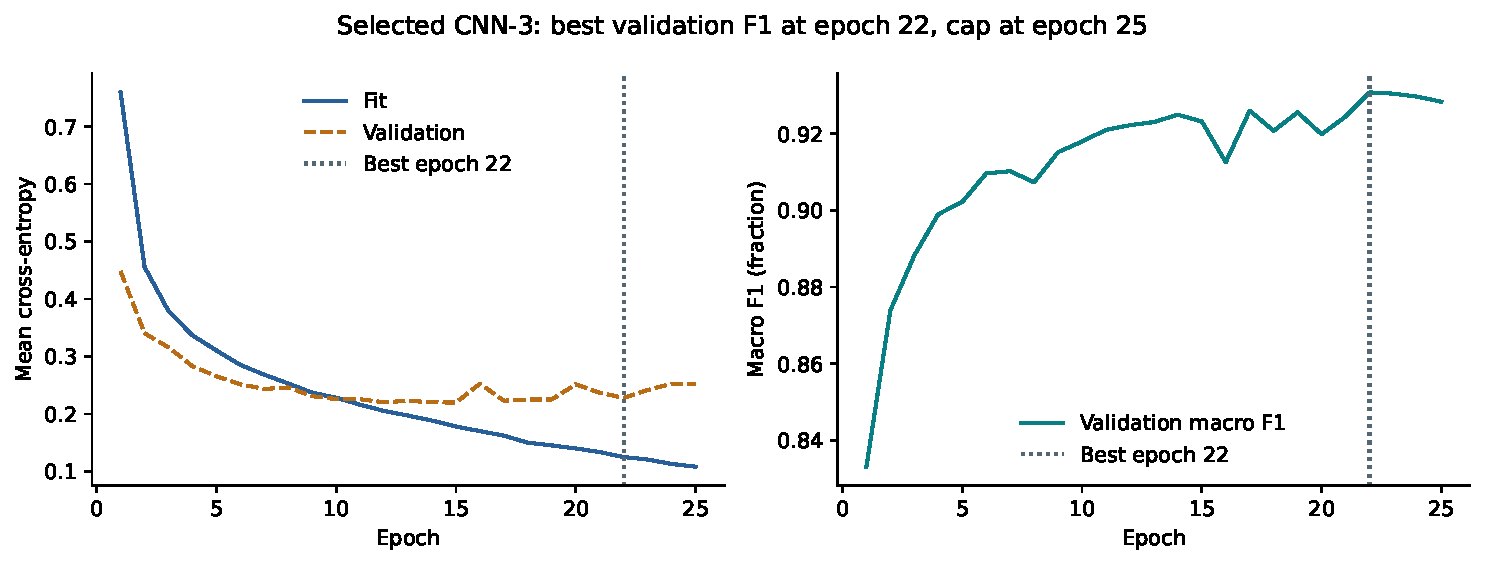
\includegraphics[width=.94\textwidth]{figures/learning.pdf}
\caption{Selected CNN-3 learning history. Epoch 22 maximizes validation macro F1;
training reaches the 25-epoch cap and reloads that checkpoint. Fit and validation
cross-entropy and validation F1 describe different criteria.}
\label{fig:learning}
\end{figure*}

Dropout $p=0.30$ is compared against zero dropout under otherwise fixed reference
settings. A legacy augmentation row shifts every fit image by independent
integer offsets in $[-2,2]$, with zero fill and unchanged frame size. The later
work-guide policy draws a shift with probability 0.5. Both evaluation and
embedding extraction use canonical images. Seed controls cover Python, NumPy,
PyTorch, shuffling and augmentation; cross-device bit-identical training is
outside the measured scope.

\section{Hybrid Method and Controls}
The selected encoder outputs $z\in\mathbb{R}^{64}$ after dense ReLU and before
dropout. HOG outputs $h\in\mathbb{R}^{1296}$ from the corresponding raw input.
The hybrid input is $[z,h]\in\mathbb{R}^{1360}$. Features are aligned by original
ID with true-label equality asserted. The encoder remains fixed while LR heads
fit on the same 48,000 examples.

Each LR pipeline fits StandardScaler on fit data, then LR with LBFGS and up to
2,000 iterations. Each feature row compares $C\in\{0.1,1\}$ by validation F1,
accuracy and C order. All chosen heads use $C=0.1$ and converged. The four rows
are the original CNN head, embedding-only LR, HOG-only LR and fusion LR.

The encoder was selected on the same validation set subsequently used to tune
the LR heads. This validation reuse supports development comparison and should
be considered when interpreting validation differences. Official-test scores
are reported only for the predeclared frozen rows. Aggregate hybrid value is
judged against both single-feature LR controls and the practical CNN row.

\section{Results}
\subsection{Validation Ablations}
Table~\ref{tab:ablations} reports the measured candidates. Against CNN-2,
removing dropout changes F1 by $-0.0036$, shifting every image by $-0.0065$,
and adding the third block by $+0.0041$. The depth comparison changes the
spatial map and dense-head size as well as the number of convolution blocks.
The common stopping rule yields different best and final epochs.

\begin{table}[t]
\caption{Validation-only CNN results, seed 42. Shirt is recall in percent;
epochs are best/final. The p50 row is the later nonselectable ablation.}
\label{tab:ablations}
\centering\scriptsize
\begin{tabular}{lrrrr}
\toprule
Configuration & F1 & Shirt & Epochs & Parameters\\
\midrule
% BEGIN GENERATED ablations
cnn2 & 0.9267 & 77.2 & 24/25 & 220,234 \\
cnn2 p0 & 0.9231 & 80.5 & 17/22 & 220,234 \\
cnn2 aug & 0.9202 & 69.1 & 25/25 & 220,234 \\
cnn3 & 0.9308 & 79.1 & 22/25 & 167,114 \\
cnn2 aug p50 & 0.9279 & 72.3 & 25/25 & 220,234 \\
% END GENERATED ablations
\bottomrule
\end{tabular}
\end{table}

The later 50\%-shift run obtains 0.9279 validation F1 versus 0.9267 for the
unaugmented reference, a $+0.0012$ change on one seed. Its Shirt recall falls
from 77.2\% to 72.3\%. Both shifted runs peak at epoch 25, so the epoch budget
may limit their conclusions. These observations provide no evidence that this
translation policy resolves Shirt confusion.

\subsection{Frozen Official-Test Comparison}
Table~\ref{tab:comparison} shows all frozen Phase 2 rows with the Phase 1 reference.
CNN-3 reaches \CnnAccuracy{} accuracy and \CnnFone{} F1. The embedding-only LR
control reaches 92.21\% and 0.9218, the highest aggregate scores among these
frozen rows. It retains its declared role as a head-control experiment. The
CNN architecture choice remains the validation-selected CNN-3.

\begin{table}[t]
\caption{Same official 10,000 test IDs. Val is validation macro F1; accuracy
and Shirt recall are percentages.}
\label{tab:comparison}
\centering\small
\begin{tabular}{lrrrr}
\toprule
Pipeline & Val & Accuracy & Test F1 & Shirt\\
\midrule
% BEGIN GENERATED comparison
HOG + SVM & 0.9114 & 90.91 & 0.9090 & 73.3 \\
CNN-3 & 0.9308 & 92.14 & 0.9207 & 71.7 \\
Embedding + LR & 0.9319 & 92.21 & 0.9218 & 74.6 \\
HOG + LR & 0.8832 & 87.60 & 0.8757 & 66.1 \\
Fusion + LR & 0.9261 & 92.06 & 0.9206 & 76.0 \\
% END GENERATED comparison
\bottomrule
\end{tabular}
\end{table}

Compared with HOG plus SVM, the CNN gains \AccuracyGain{} percentage points
accuracy and \FoneGain{} macro F1. The paired bootstrap uses 2,000 aligned-ID
resamples, seed 42, and gives a 95\% accuracy-gain interval of
$[+\AccCiLower{},+\AccCiUpper{}]$ percentage points. Its F1-gain interval is
$[+0.0067,+0.0170]$. These intervals concern benchmark-sample variability.
Training-seed variability is unmeasured.

Fusion has validation F1 0.9261 versus 0.9319 for embedding-only LR. Test F1
is 0.9206 versus 0.9218. Fusion therefore adds complexity without an aggregate
benefit in this pipeline. Its 76.0\% test Shirt recall is a descriptive class
trade-off observed after freeze, with no validation-based rule selecting it
for that objective.

\subsection{Class Recall and Paired Mistakes}
Table~\ref{tab:recall} reports the complete class recall comparison. Shirt
remains the weakest CNN category at \CnnShirt{}, down from \SvmShirt{}.
Shirt precision rises from 75.2\% to 80.9\% and Shirt F1 rises from 0.742 to
0.760. The CNN sends 134 true Shirts to T-shirt/top versus 103 for SVM, while
sending 64 true T-shirts to Shirt versus 104 for SVM. This changes the
precision/recall trade-off between similar categories.

\begin{table}[t]
\caption{Official-test recall, 1,000 examples per true category. Delta is CNN
minus SVM in percentage points.}
\label{tab:recall}
\centering\small
\begin{tabular}{lrrr}
\toprule
Category & SVM (\%) & CNN (\%) & Delta\\
\midrule
% BEGIN GENERATED recalls
T-shirt/top & 85.7 & 90.6 & +4.9 \\
Trouser & 97.6 & 99.0 & +1.4 \\
Pullover & 86.2 & 89.7 & +3.5 \\
Dress & 91.2 & 92.1 & +0.9 \\
Coat & 86.4 & 87.3 & +0.9 \\
Sandal & 96.5 & 98.6 & +2.1 \\
Shirt & 73.3 & 71.7 & -1.6 \\
Sneaker & 97.3 & 98.3 & +1.0 \\
Bag & 98.3 & 98.6 & +0.3 \\
Ankle boot & 96.6 & 95.5 & -1.1 \\
% END GENERATED recalls
\bottomrule
\end{tabular}
\end{table}

Across all test IDs, both models are correct on 8,789 images. Only the CNN is
correct on 425, only the SVM on 302, and both fail on 484. Thus
$(425-302)/10000=0.0123$, exactly the accuracy gain. The exact McNemar test
on 727 discordant pairs gives $p=5.8\times10^{-6}$. It is a paired comparison
on the same benchmark and omits training-seed variation.

\begin{figure*}[t]
\centering
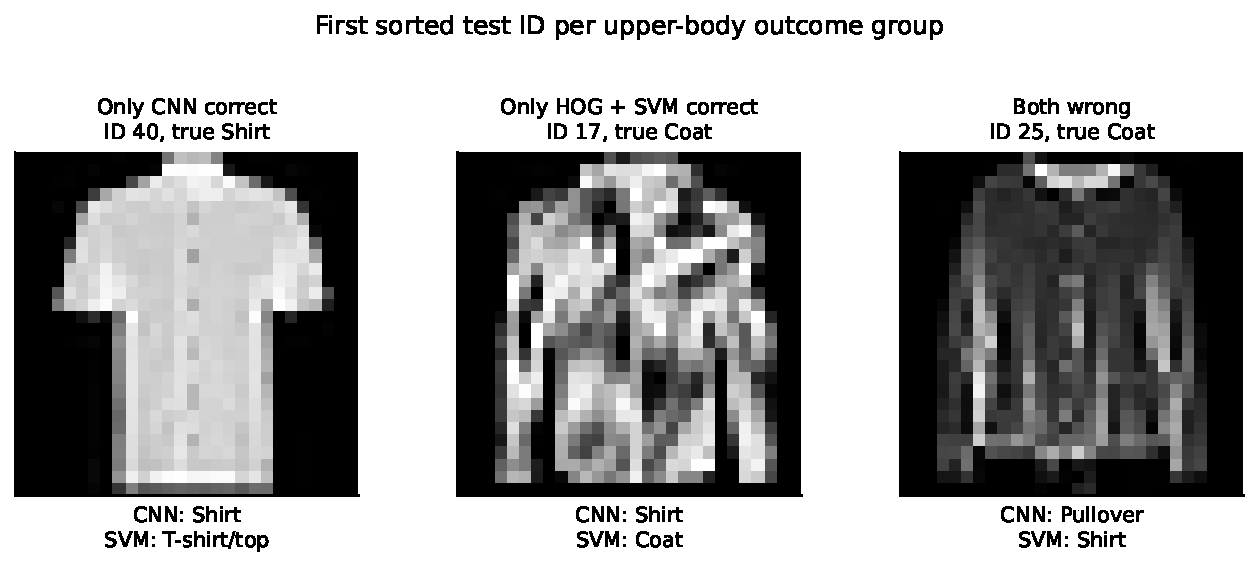
\includegraphics[width=.85\textwidth]{figures/errors.pdf}
\caption{First sorted original test ID within three upper-body outcome groups.
Captions show observed labels and paired predictions. Visible fastenings or
outlines suggest hypotheses, with no causal attribution from a single image.}
\label{fig:errors}
\end{figure*}

\section{Inference Cost, Complexity and Reproducibility}
The recorded final benchmark uses one Apple M3 CPU, PyTorch 2.15.0 and native
thread limits of one. It evaluates raw official-test IDs 0--1023 in batches of
128, with one warm-up and five repeats. Timing includes input conversion,
feature extraction, scaling and prediction with loaded models. Table~\ref{tab:timing}
reports amortized batch cost. Disk I/O and model loading lie outside the timed
interval. The recorded legacy SVM refit reproduced all 10,000 saved predictions
before its same-machine timing measurement.

\begin{table}[t]
\caption{Recorded same-machine CPU end-to-end cost, ms/image. Range spans the
five repeated batch measurements.}
\label{tab:timing}
\centering\small
\begin{tabular}{lrr}
\toprule
Pipeline & Median & Range\\
\midrule
% BEGIN GENERATED timing
HOG + SVM & 19.748 & 19.302--19.902 \\
CNN-3 & 0.312 & 0.293--0.421 \\
Embedding + LR & 0.315 & 0.294--0.393 \\
HOG + LR & 0.205 & 0.204--0.215 \\
Fusion + LR & 0.518 & 0.515--0.554 \\
% END GENERATED timing
\bottomrule
\end{tabular}
\end{table}

CNN cost is \CnnTime{} ms/image versus \SvmTime{} for SVM, a ratio of
\SpeedRatio{}. Fusion costs 0.518 ms/image. The CNN has 167,114 trainable values
and a 673,525-byte torch checkpoint. SVM stores 27,295,425 decision-array
scalars plus scaler statistics, a storage proxy with a different meaning.
Embedding LR adds 650 head values and ships the fixed 166,464-value encoder.
Fusion adds 13,610 LR values and the same encoder. Serialized formats and
compression differ, so file size is labeled alongside each artifact.

The integrated notebook independently derives metrics from integer confusion
counts for 31 full-profile prediction files, including all six fusion-head
candidates and the later augmentation row. It checks original ID membership,
authoritative labels, stored metric equality and frozen artifact hashes.
After integration, all 60 tests pass and the selected CNN checkpoint reproduces
all 12,000 validation predictions. Sources, configs, predictions, learning
histories and manifests remain in the repository at
\url{https://github.com/Nakul-Jaglan/aml-dl-t089}.

\section{Limitations and Conclusion}
The comparison uses one training seed, one saved split and a compact model
search. Near-copy findings and prior Phase 1 test examination limit how the
public benchmark should be interpreted. Small centered grayscale images do
not establish recognition under arbitrary backgrounds or camera conditions.
The bootstrap omits training-seed variation, and timing is specific to the
recorded machine and implementation. Qualitative error explanations remain
hypotheses.

The learned representation improves aggregate clothing recognition under the
recorded protocol. CNN-3 reaches \CnnAccuracy{} accuracy and \CnnFone{} macro F1,
with lower measured CPU batch cost than the classical SVM. Shirt recall falls,
showing why per-class analysis matters. The optional fusion is technically
implemented and controlled, while its aggregate result provides no evidence
of additional value over embedding-only LR. These findings support a bounded,
reproducible account of the completed Phase 2 experiment.

\bibliographystyle{IEEEtran}
\bibliography{references}
\end{document}
